
\documentclass[a4paper]{article}
\usepackage[margin=0.75in]{geometry} % margins
\usepackage[english]{babel}
\usepackage[utf8]{inputenc}
\usepackage{amsmath}
\usepackage{graphicx}
\usepackage[colorinlistoftodos]{todonotes}
\usepackage{float} % Image float [H] option
\usepackage{subfig} % Figures in figures ( I think)

\usepackage[square]{natbib}

\usepackage{hyperref} % \url

% Default Font
\usepackage[default]{lato}
\usepackage[T1]{fontenc}
\renewcommand{\mddefault}{l}% switch default weight to light

% Paragraphs
\setlength{\parskip}{\baselineskip}	% add space between paragraphs
\setlength{\parindent}{0pt}			    % No paragraph indent
\usepackage[none]{hyphenat}         % No Hyphens

% Declare first level dot point as a -
\def\labelitemi{--}

% Smart quotes
\usepackage [autostyle, english = american]{csquotes}
\MakeOuterQuote{"}

%pdf
\usepackage{pdfpages}
\title{Object Oriented - Project 2: Shadow Quest}

\author{James Stone - 761353}

\date{October 2016}

\begin{document}
\maketitle

\section{Reflection}

\subsection{Changes made}

Rather than follow my design for the assignment from Part A, I decided to model my solution off the sample solution.
I followed this design closely with no major changes. I did however make some minor changes to a few private fields were removed such as:
\begin{description}
\item[\texttt{attacked}]from the \texttt{Unit} class
\item[\texttt{talking}]from the \texttt{NPC} class
\end{description}
These were instead replaced by a private method called \texttt{underAttack} and \texttt{talking}. The advantage of this was it was one less field I had to keep updated, and they both could be represented through a simple calculation from other fields \texttt{attackTime <= 0} and \texttt{talkingtime <= 0}
\subsubsection{Class diagram}

Please see the next page for the Class diagram.

And then the following page for the rest of the reflection.

Note: the class Diagram was modified from the Sample Solution.
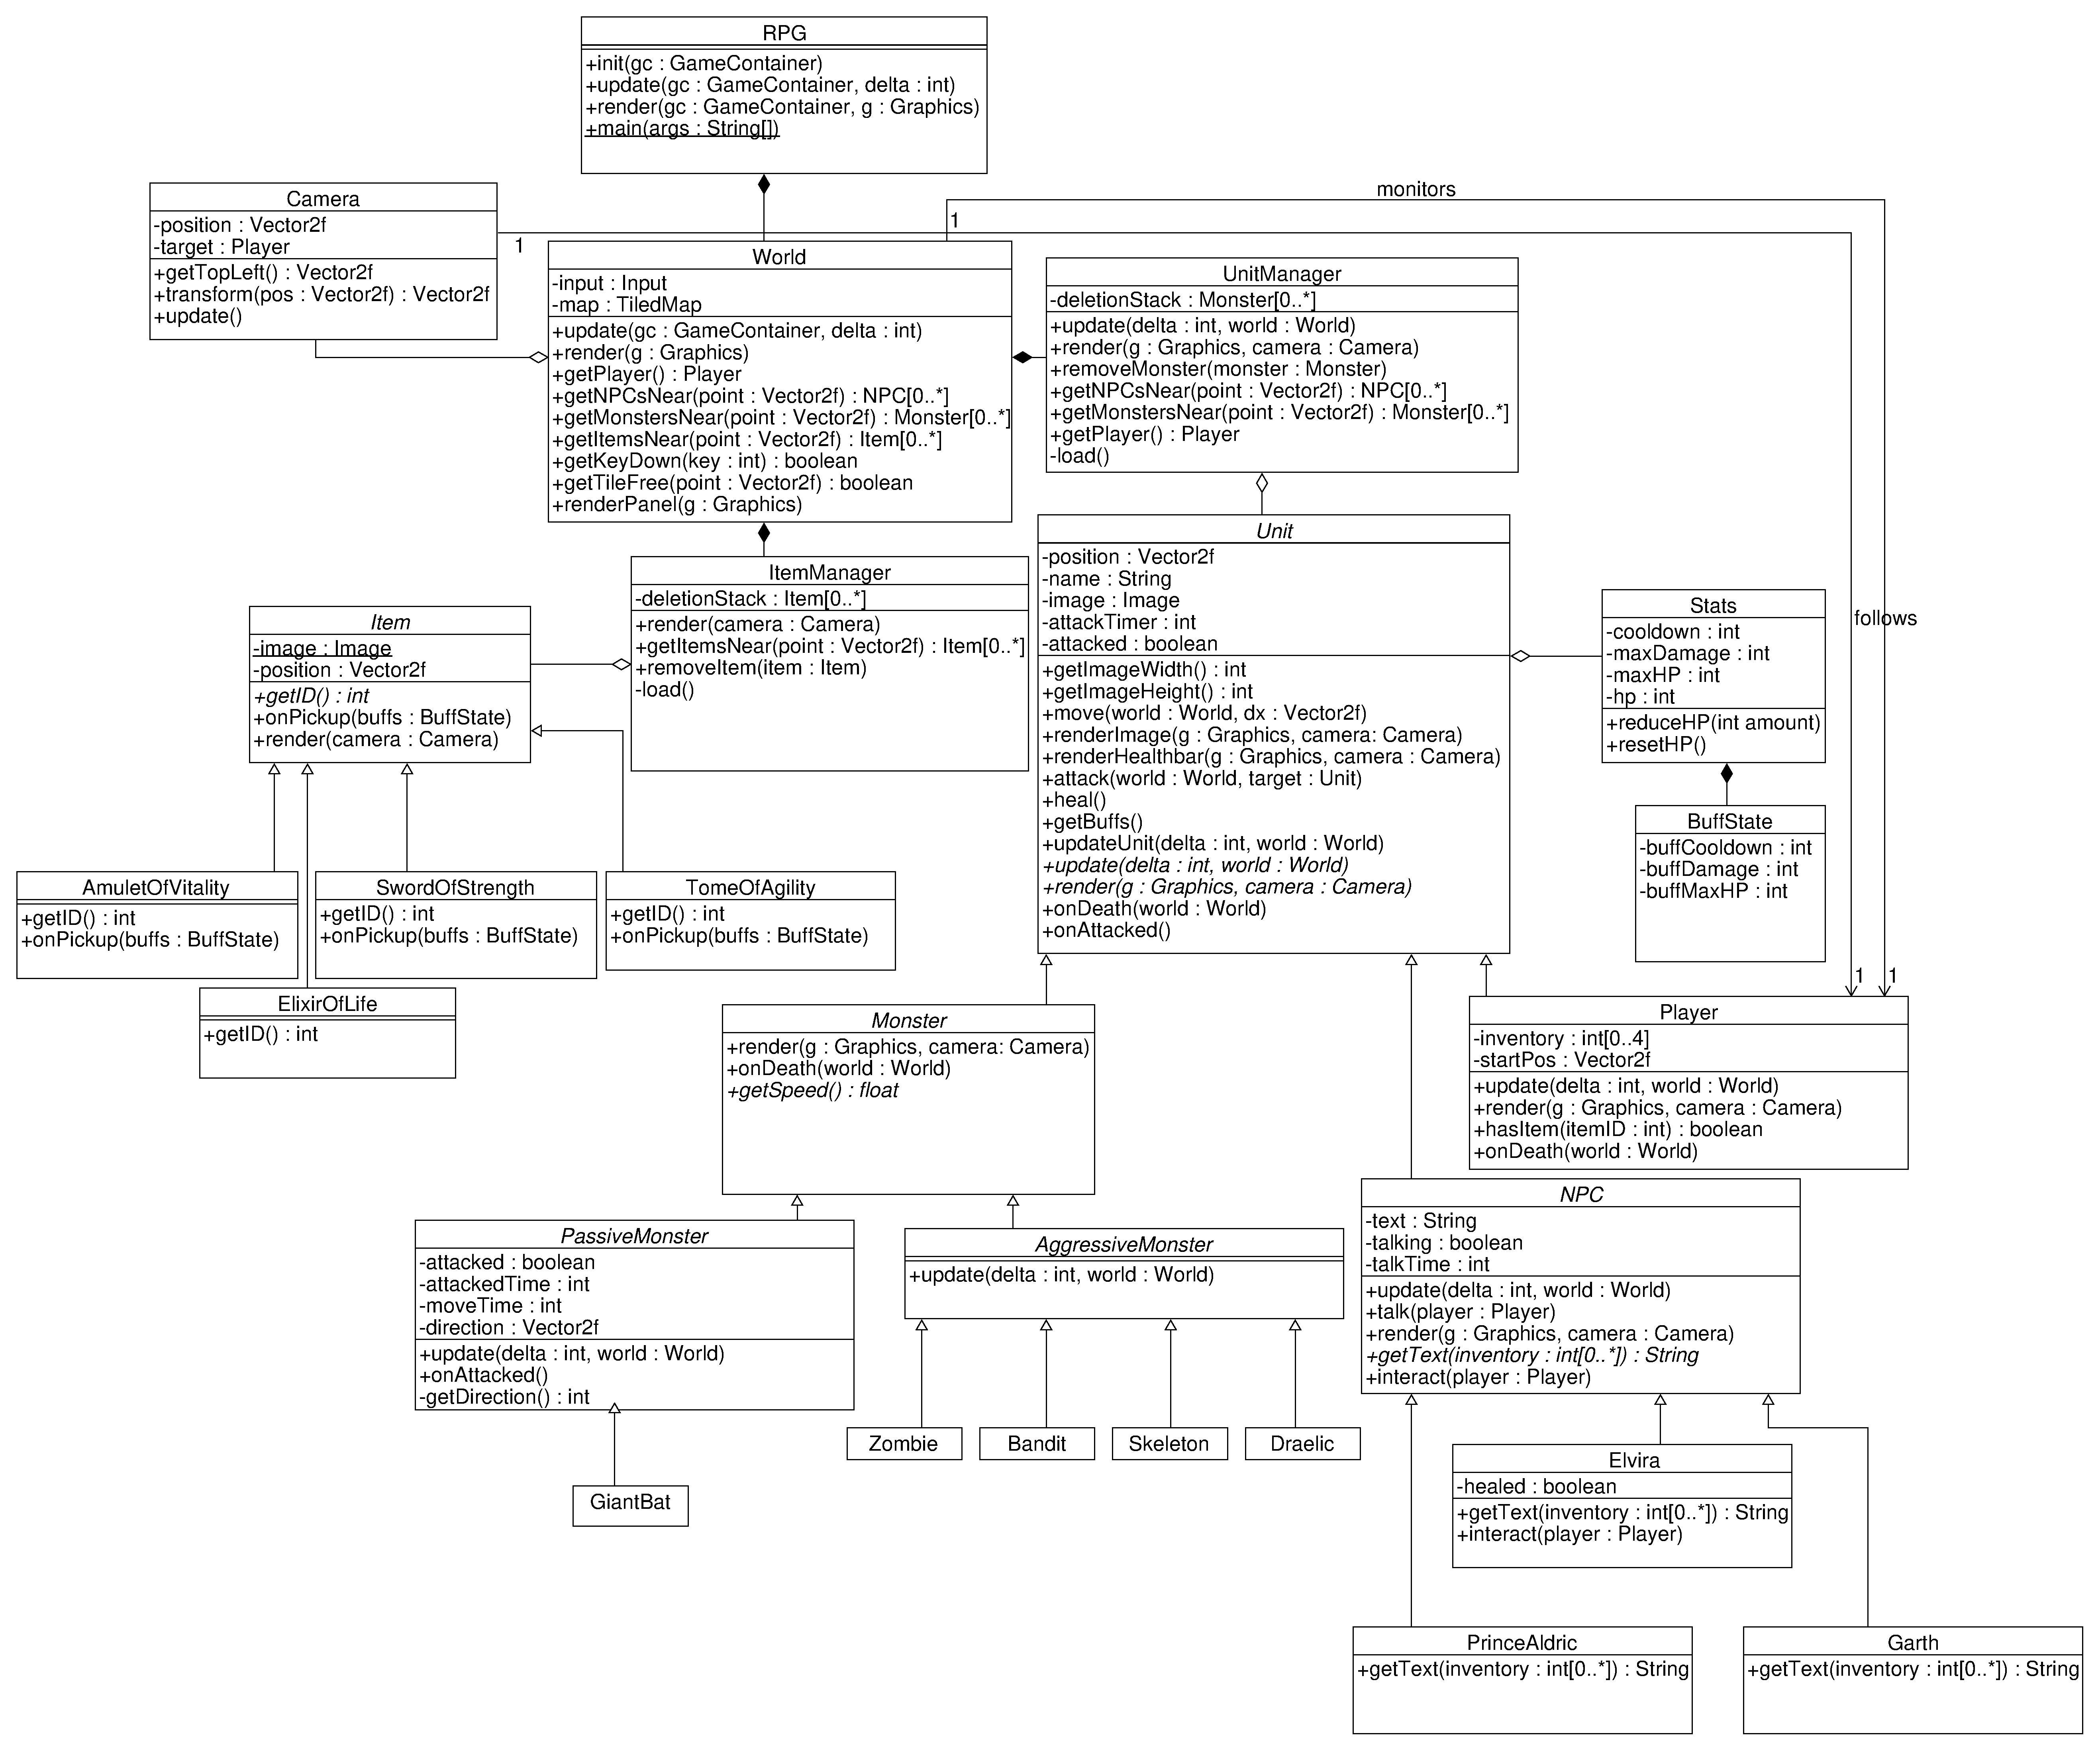
\includepdf[landscape=true]{UML.pdf}


\subsection{Knowledge gained}
I really enjoyed this assignment, it's really been an eye opener for me into how beneficial the Object oriented paradigm can be.
It really maximises the amount of code re-usability, and all the advantages that come with that:
\begin{itemize}
\item less development time
\item less bugs
\item easier to test as more modular and abstract
\end{itemize}

This was really highlighted to me most when I had a bug in my \texttt{move} method of the \texttt{Unit} class. Once i fixed this bug suddenly all of my Monsters and the player could move again.

\subsection{What I would do differently}
If I was to do this again I would consider making the \texttt{statusPanel} its own class. To me it seems rather odd having it attached to a \texttt{world}, when the status panel relates to a \texttt{player} and there is one \texttt{statusPanel} per \texttt{RPG}.
I would also consider making the \texttt{inventory} its own class. Alternatively I'd consider using an \textt{ItemManager} as a \texttt{player}'s inventory

\end{document}
